\documentclass[paper=letter,fontsize=11pt]{scrartcl} % KOMA-article class
							
\usepackage[english]{babel}
\usepackage[utf8x]{inputenc}
\usepackage[protrusion=true,expansion=true]{microtype}
\usepackage{amsmath,amsfonts,amsthm}     % Math packages
\usepackage{graphicx}                    % Enable pdflatex
\usepackage[svgnames]{xcolor}            % Colors by their 'svgnames'
\usepackage{geometry}
	%\textheight=700px                    % Saving trees ;-)
%\usepackage{url}
\usepackage[colorlinks=true,
linkcolor=blue,
urlcolor=blue]{hyperref}
\usepackage{float}
\usepackage{etaremune}
\usepackage{wrapfig}

\usepackage{attachfile}
\usepackage{mfirstuc} % Title letters
\MFUnocap{in}

\setlength\topmargin{0pt}
\addtolength\topmargin{-\headheight}
\addtolength\topmargin{-\headsep}
\setlength\oddsidemargin{0pt}
\setlength\textwidth{\paperwidth}
\addtolength\textwidth{-2in}
\setlength\textheight{\paperheight}
%\addtolength\textheight{-3in}
\addtolength\textheight{-2in}
\usepackage{layout}

\usepackage{fancyhdr} % personalize foot and page number
\pagestyle{fancy}
\fancyhf{}
\renewcommand{\headrulewidth}{0pt}
\fancyfoot[R]{Dechao Tian, Ph.D. Page \thepage}

%\addtolength{\voffset}{-40pt}
%\addtolength{\textheight}{20pt}


%%% Custom sectioning}{sectsty package)
%%% ------------------------------------------------------------
\usepackage{sectsty}

\sectionfont{%			            % Change font of \section command
	\usefont{OT1}{phv}{b}{n}%		% bch-b-n: CharterBT-Bold font
	\sectionrule{0pt}{0pt}{-7pt}{1pt}}
%%% Macros
%%% ------------------------------------------------------------
\newlength{\spacebox}
\settowidth{\spacebox}{8888888888}			% Box to align text
\newcommand{\sepspace}{\vspace*{1em}}		% Vertical space macro

\newcommand{\MyName}[3]{ % Name
    \noindent \Huge \usefont{OT1}{phv}{b}{n} #1 \\ \\
        \noindent \normalsize \normalfont
     %   \vspace{\parskip}
        \begin{minipage}[t]{0.48\textwidth} \textit{#2} \end{minipage}
            \hfill
        \begin{minipage}[t]{0.48\textwidth} \begin{flushright} \textit{#3} \end{flushright} \end{minipage}
            }
%        \parbox[t][3cm][t]{7cm}{\noindent #2} \hfill
%        \parbox[t][3cm][t]{7cm}{\noindent #3}
%        \noindent \normalsize \normalfont #2
%		\colorbox{White}{%
%			\parbox{20em}{%
%			\hfill\color{Black}#3}} \par  % Duration
%\newcommand{\MyName}[1]{ % Name
%		\Huge \usefont{OT1}{phv}{b}{n} \hfill #1
%		\par \normalsize \normalfont}
		
\newcommand{\MySlogan}[1]{ % Slogan}{optional)
		\large \usefont{OT1}{phv}{m}{n}\hfill \textit{#1}
		\par \normalsize \normalfont}

\newcommand{\NewPart}[2]{\section*{\capitalisewords{#1} #2}}

\newcommand{\PersonalEntry}[2]{
		\noindent\hangindent=2em\hangafter=0 % Indentation
		\parbox{\spacebox}{        % Box to align text
		\textit{#1}}		       % Entry name}{birth, address, etc.)
		\hspace{1.5em} #2 \par}    % Entry value

\newcommand{\SkillsEntry}[2]{      % Same as \PersonalEntry
    \noindent \textbf{#1} \par #2 \par }

\newcommand{\TeachEntry}[1]{      % Same as \PersonalEntry
    \noindent #1 \par }
		
\newcommand{\EducationEntry}[4]{
		\noindent \textbf{#1} \hfill      % Study
		\colorbox{White}{%
			\parbox{10em}{%
			\hfill\color{Black}#2}} \par  % Duration
		\noindent \textit{#3} \par        % School
		\noindent\hangindent=2em\hangafter=0 \small #4 % Description
		\normalsize \par}

\newcommand{\WorkEntry}[4]{				  % Same as \EducationEntry
		\noindent \textbf{#1} \hfill      % Jobname
		\colorbox{White}{\color{White}#2} \par  % Duration
		\noindent \textit{#3} \par              % Company
		\noindent\hangindent=2em\hangafter=0 \small #4 % Description
		\normalsize \par}

\newcommand{\PaperEntry}[7]{
		\noindent #1, #2, \textit{#3} \textbf{#4}, #5 (#6).}
		%\noindent #1, \href{#7}{#2}, \textit{#3} \textbf{#4}, #5 (#6).}

\newcommand{\ManEntry}[2]{
		\noindent #1, #2.}

\newcommand{\ArxivEntry}[3]{
		\noindent #1, ``\href{http://arxiv.org/abs/#3}{#2}", \textit{{cond-mat/}#3}.}
        
\newcommand{\PosterEntry}[3]{
    \noindent #1, #2, #3}

\newcommand{\ExperienceEntry}[4]{
		\noindent \textbf{#1} \hfill      % Study
		\colorbox{White}{%
			\parbox{10em}{%
			\hfill\color{Black}#2}} \par  % Duration
		\noindent \textit{#3}         % School
		\noindent\hangindent=2em\hangafter=0 \small #4 % Description
		\normalsize}

\newcommand{\BookEntry}[4]{
		\noindent #1, ``\href{#3}{#4}", \textit{#3}.}
        
\newcommand{\FundingEntry}[5]{
        \noindent #1, ``#2", \$#3 (#4, #5).}

\newcommand{\TalkEntry}[4]{
		\noindent #1, #2, #3 #4}

\newcommand{\ThesisEntry}[5]{
		\noindent #1 -- #2 #3 ``#4" \textit{#5}}

\newcommand{\CourseEntry}[3]{
		\noindent \item{#1: \textbf{#2} \\ #3}}

\newcommand{\ReferenceEntry}[3]{
        \noindent \textbf{#1} \par 
        \noindent #2 \par
        \noindent \underline{\textit{Contact Information}} \par
        \noindent #3 \par }

%%% Begin Document
%%% ------------------------------------------------------------
\begin{document}
\thispagestyle{empty}

%\layout

% you can upload a photo and include it here...
%\begin{wrapfigure}{l}{0.5\textwidth}
%	\vspace*{-2em}
%		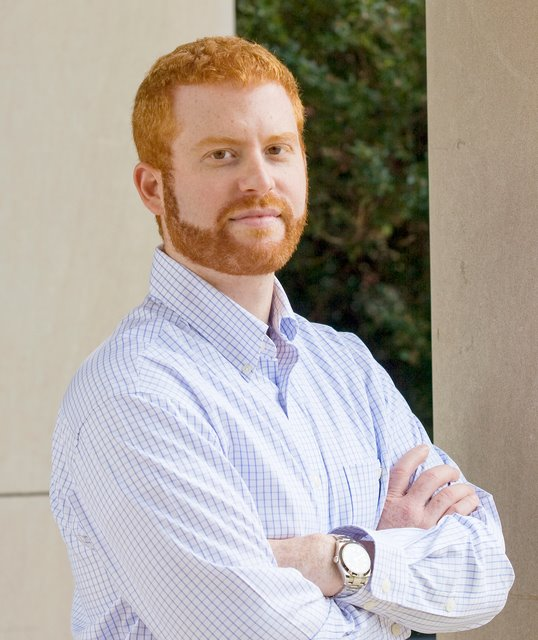
\includegraphics[width=0.2\textwidth]{Appelbaum.JPG}
%\end{wrapfigure}

\MyName{Dechao Tian}{5000 Forbes Ave GHC 7415 \\
Pittsburgh, PA, 15213 \\
}{(412) 583-6800\\
dechaot@andrew.cmu.edu\\https://tian-dechao.github.io}

%\sepspace

%\NewPart{Overview}{}
% Professor of Physics, APS Fellow, Condensed Matter Experiment {\em and} Theory.
\NewPart{Current employment}{}
\EducationEntry{Postdoctoral Research Associate}{2015 - Present}{Carnegie Mellon University}
{\begin{itemize}\item{Computational Biology Department, Ma Laboratory - Computational Genomics: research on regulatory network, systems biology, and 3D chromatin organization }\end{itemize}}

%%% Education
%%% ------------------------------------------------------------
\NewPart{Education}{}

\EducationEntry{Ph.D. in Statistics and Applied Probability}{2010 - 2015}{National University of Singapore, Singapore}{Thesis title: Biological Network Analysis and Comparison\\
Thesis advisor: Dr. Kwok Pui Choi}
%Thesis advisor: Dr. Louxin Zhang and Dr. Kwok Pui Choi}
\sepspace
\EducationEntry{M.S. in Probability and Mathematical Statistics}{2009 - 2011}{Northeast Normal University, China}{Thesis title: Random Network Models' Discrimination \\
Thesis advisor: Dr. Zhidong Bai}
\sepspace
\EducationEntry{B.S. in Mathematics and Applied Mathematics}{2005 - 2009}{Northeast Normal University, China}{}

\NewPart{Manuscripts in Preparation}{}
\begin{etaremune}
\item \ManEntry{\textbf{Tian D}$^\star$, Zhang R$^\star$, Zhang Y, and Ma J}{MOCHI enables discovery of heterogeneous interactome modules in cell nucleus}
\item \ManEntry{\textbf{Tian D}$^\star$, Zhu X$^\star$, and Ma J}{Diffdomains: model-based identification of significantly reshaped chromatin domains from Hi-C contact matrices between normal and disease conditions}
\item \ManEntry{\textbf{Tian D} and Ma J}{Exploiting the interplay between chromatin interactome and transcriptional regulatory network}
\end{etaremune}

\NewPart{Publications}{}
\begin{etaremune}
\item \PaperEntry{\textbf{Tian D}, Gu Q and Ma J}{Identifying gene regulatory network rewiring using latent differential graphical models}{Nucleic Acids Research}{44}{17}{2016}{https://academic.oup.com/nar/article/44/17/e140/2468041}  
\item \PaperEntry{Koh V, Cheung C, Li X, \textbf{Tian D}, Wang J.J, Mitchell P, Cheng C.Y, and Wong T.T}{Retinal vein occlusion in a multi-ethnic asian population: the singapore epidemiology of eye disease study}{Ophthalmic Epidemiology}{23}{1}{2016}{https://www.tandfonline.com/doi/abs/10.3109/09286586.2015.1082604}
%\item \PaperEntry{Chen et al. (including \textbf{Tian D})}{Plasma metabonomic profiling of diabetic retinopathy}{Diabetes}{65}{4}{2016}{http://diabetes.diabetesjournals.org/content/early/2016/01/14/db15-0661.short}
\item \PaperEntry{Chen L, Cheng C.Y, Choi H, Ikram M.K, Sabanayagam C, Tan G.S, \textbf{Tian D}, Zhang L, Venkatesan G, Tai E.S, Wang J.J, Mitchell P, Cheung C.M.G, Beuerman R.W, Zhou L, Chan E.C.Y, Wong T.T}{Plasma metabonomic profiling of diabetic retinopathy}{Diabetes}{65}{4}{2016}{http://diabetes.diabetesjournals.org/content/early/2016/01/14/db15-0661.short}
%\item \PaperEntry{Yam et al. (includiing \textbf{Tian D})}{Ex vivo propagation of human corneal stromal ``activated keratocytes" for tissue engineering}{Cell Transplantation}{24}{9}{2015}{https://www.ingentaconnect.com/content/cog/ct/2015/00000024/00000009/art00013}
\item \PaperEntry{Yam G.H.F, Yusoff N.Z.B.M, Kadaba A, \textbf{Tian D}, Myint H.H,  Beuerman R.W, Zhou L, Mehta J.S}{Ex vivo propagation of human corneal stromal ``activated keratocytes" for tissue engineering}{Cell Transplantation}{24}{9}{2015}{https://www.ingentaconnect.com/content/cog/ct/2015/00000024/00000009/art00013}
%\item \PaperEntry{Chen et al. (including \textbf{Tian D})}{Global metabonomic and proteomic analysis of human conjunctival epithelial cells (IOBA-NHC) in response to hyperosmotic stress}{Journal of Proteome Research}{14}{9}{2015}{https://pubs.acs.org/doi/abs/10.1021/acs.jproteome.5b00443}
\item \PaperEntry{Chen L, Li J, Guo T, Ghosh S, Koh S.K, \textbf{Tian D}, Zhang L, Jia D, Beuerman R.W, Aebersold R, Chan E.C.Y, Zhou L}{Global metabonomic and proteomic analysis of human conjunctival epithelial cells (IOBA-NHC) in response to hyperosmotic stress}{Journal of Proteome Research}{14}{9}{2015}{https://pubs.acs.org/doi/abs/10.1021/acs.jproteome.5b00443}
%\item \PaperEntry{Tong et al. (including  \textbf{Tian D})}{Quantitation of 47 human tear proteins using high resolution multiple reaction monitoring (HR-MRM) based-mass spectrometry}{Journal of Proteomics}{115}{}{2015}{https://www.sciencedirect.com/science/article/pii/S1874391914005557}
\item \PaperEntry{Tong L, Zhou X, Jylha A, Aapola U, Liu D.N, Koh S.W, \textbf{Tian D}, Quah J, Uusitalo H, Beuerman R.W, Zhou L}{Quantitation of 47 human tear proteins using high resolution multiple reaction monitoring (HR-MRM) based-mass spectrometry}{Journal of Proteomics}{115}{}{2015}{https://www.sciencedirect.com/science/article/pii/S1874391914005557}
\item \PaperEntry{Zhang S$^\star$, \textbf{Tian D}$^\star$,  Tran N.H, Choi K.P, and Zhang L.X}{Profiling human cell-type specific transcription factor regulatory networks}{Nucleic Acids Research}{42}{20}{2014}{https://academic.oup.com/nar/article/42/20/12380/2902979}  
%\item \PaperEntry{Barathi et al. (including \textbf{Tian D})}{Involvement of GABA transporters in atropine-treated myopic retina as revealed by iTRAQ quantitative proteomics}{Journal of Proteome Research}{13}{11}{2014}{https://pubs.acs.org/doi/abs/10.1021/pr500558y}
\item \PaperEntry{Barathi V.A, Chaurasia S.S, Poidinger M, Koh S.K, \textbf{Tian D}, Ho C, Iuvone P.M, Beuerman R.W, Zhou L}{Involvement of GABA transporters in atropine-treated myopic retina as revealed by iTRAQ quantitative proteomics}{Journal of Proteome Research}{13}{11}{2014}{https://pubs.acs.org/doi/abs/10.1021/pr500558y}
\item \PaperEntry{\textbf{Tian D} and Choi K.P}{Sharp bounds and normalization of wiener-type indices}{PLOS ONE}{8}{11}{2013}{https://journals.plos.org/plosone/article?id=10.1371/journal.pone.0078448}
%\par \sepspace \noindent  \underline{\textit{Manuscripts in preparation}}
%\item \ManEntry{\textbf{Tian D}$^\star$, Zhang R$^\star$, Zhang Y, and Ma J}{MOCHI enables discovery of heterogeneous interactome modules in cell nucleus}
%\item \ManEntry{\textbf{Tian D} and Ma J}{Exploiting the interplay between chromatin interactome and transcriptional regulatory network}
%\item \ManEntry{\textbf{Tian D}$^\star$, Zhu X$^\star$, and Ma J}{Diffdomains: model-based identification of significantly reshaped chromatin domains from Hi-C contact matrices between different biological conditions}
\end{etaremune}
~~~~~ Note: $\star$ represents co-first authors.

\NewPart{Research experience}{}
\begin{etaremune}
\item \ExperienceEntry{National University of Singapore, Singapore}{2014 - 2015}{Research Assistant. Advisor: Kwok Pui Choi, Ph.D.}{\begin{itemize} \item Develop model to identify essential genes by network motifs in regulatory networks \end{itemize}}
\item \ExperienceEntry{Singapore Eye Research Institute (SERI), Singapore}{2011 - 2015}{Research Collaborator with Lei Zhou, Ph.D.
}{\begin{itemize} 
    \item Provide statistical analysis and consultation for
     Proteomics $\&$ Microanalysis Laboratory
    \item Collaborate with other members from SERI \end{itemize}}
\item \ExperienceEntry{Center for Quantitative Medicine, Duke-NUS, Singapore}{2012 - 2015}{Associate Member}{}
\end{etaremune}

\NewPart{Teaching assistant}{}
\TeachEntry{ST1131 Introduction to Statistics}
\TeachEntry{ST1232 Statistics for Life Science}
\TeachEntry{ST2131 Probability}

\NewPart{Skills}{}
\SkillsEntry{Programming (Most used first)}{R, Python, Unix/Linux bash script command, SAS programming language (Certified Base Programmer for SAS 9)}
%\SkillsEntry{Statistics}{Sample size computation and power analysis, Hypothesis test, Random matrix theory}
\SkillsEntry{Bioinformatics tools \& databases}{
    MEME Suite, bedtools, jucier, UCSC Genome Browser, ENCODE, TCGA }

\NewPart{Posters}{}
\begin{etaremune}
\item  \PosterEntry{Systems Biology, Global Regulation $\&$ Gene Expression}{CSHL}{2018}
\item  \PosterEntry{4DN Annual Meeting}{NIH}{2017}
\end{etaremune}

\NewPart{References}{}
\ReferenceEntry{Jian Ma, Ph.D.}{Associate Professor, Computational Biology\\Carnegie Mellon University}{School of Computer Science\\ Carnegie Mellon University\\ 5000 Forbes Avenue \\Pittsburgh, PA 15213, USA\\Tel:(412) 268-2776\\jianma@cs.cmu.edu}
\sepspace
\ReferenceEntry{Louxin Zhang, Ph.D.}{Professor, Mathematics\\ National University of Singapore, Singapore}{10 Lower Kent Ridge, Singapore 119076\\Tel:(+65) 6516-6579\\matzlx@nus.edu.sg}
\sepspace
\ReferenceEntry{Kwok Pui Choi, Ph.D.}{Associate Professor, Statistics\\ National University of Singapore, Singapore}{National University of Singapore, 6 Science Drive 2, Singapore 117546\\Tel:(+65) 6516-4387\\stackp@nus.edu.sg}
\sepspace
\ReferenceEntry{Zhidong Bai, Ph.D.}{Professor, Probability\\ Northeast Normal University, China}{Shool of Mathematics and Statistics\\Northeast Normal University \\5268 Renmin Street, Changchun, Jilin 130024, China\\Tel:(+86) 0431-85098161\\baizd@nenu.edu.cn}
\end{document}
